\section{Methodology}
The core database in the system is a content registry, indexed by content-producing organization~(CPO) with the perceptual hashes of content. The lifecycle of watermark creation consists of the content producing organization calculating perceptual hashes for all their content, encrypting those perceptual hashes to an MP-FHE encryption key for the database, and then digitally signing those encrypted perceptual hashes to establish provenance. Then, when users want to query the provenance of some potentially modified image, they request the parties running the MP-FHE database to find the images with the lowest Hamming distance, then are returned the most likely sources for the image. If no nearby matches are found, then the system falls back to the na\"ive AI image classifier model. 

\subsection{Perceptual Hash Design}

\citet{oquab2023dinov2} developed DINOv2, a self-supervised feature-extracting ViT network that is trained to generate feature vectors invariant to crops and natural perturbations like color jittering, gaussian blur and solarization.

We use the pre-trained DINOv2 ViT-B/14~(with register tokens) to extract feature embeddings of the given image. Then, we apply PCA to de-correlate each component of the feature vector and simultaneously reduce the dimensionality of the feature vector from $768$ to $96$, then apply the LSH step to obtain a $96$-bit binary string. Naturally, the resulting binary string serves the purpose of a perceptual hash since the original feature vector is highly robust to perceptual transformations of the image. We also implement our own adversarial training scheme, which is discussed in detail in \autoref{sec:adversarial}.

\noindent\textbf{Statistical Test.}
Let $H\in \{ 0,1 \}^{k}$ be the hash of an image $x$ in the database of the CPO that we wish to compare the query image against and, $H'$, be the corresponding hash of a query image $x'$. The detection test compares the number of matching bits between $H$ and $H'$ to a threshold, i.e. if
\begin{equation} 
M\left(H,H'\right) \geq \tau \,\,\textrm{ where }\,\, \tau\in 
\{0,\ldots,k\}, %\vspace{-0.3cm}
\end{equation}
then the two images are considered to be the same.

For the case where $x$ and $x'$ do not correspond to same image, we assume that bits $h_1,\ldots, h_k$ are i.i.d.  Bernoulli random variables with parameter $0.5$. Then $M(H, H')$ follows a binomial distribution with parameters~($k$, $0.5$).
% The binomial distribution can be approximated by the normal distribution $\mathcal{N}(0.5,\,\frac{0.25}{k})$ when $k$ is large. 

The False Positive Rate~(FPR) is the probability that $M(H, H')$ takes a value bigger than the threshold $\tau$.
\begin{align}
\label{eq:fpr}
    % \text{FPR}(\tau) & = \mathbb{P}\left(M \geq \tau \right) \approx \phi \left( \frac{0.5-\tau}{\sqrt{\frac{0.25}{k}}}\right). 
\text{FPR}(\tau) &= P(X \geq \tau), \quad X \sim \text{Binomial}(k, 0.5)
\end{align}

% Where $\phi$ denotes the cumulative density function of the standard normal variable.
% In the case of comparison against multiple images, we compare the hash $H'$ of the query image to the other hashes $ \left( H_{1},\dots, H_{N} \right)$. %
% There are now $N$ hypotheses to test, and if all are rejected, we conclude that the image was produced by the CPO.
% The FPR for this joint hypothesis for a given threshold $\tau$ is given by:
% \vspace{-0.2cm}
% \begin{equation}\label{eq:globalFPR}
%     \text{FPR}(\tau,N) = 1-(1-\text{FPR}(\tau))^N\approx N \cdot \text{FPR}(\tau).
% \vspace{-0.2cm}
% \end{equation}
Varying $\tau$ necessitates a trade-off between the False Negative Rate~(FNR) and the FPR, which can be set according to the sensitivity of the use case.

\subsection{Preserving Privacy of End-Users}
\noindent{\textbf{Problem Definition.}} In many real-world scenarios, maintaining a perceptual hash database poses significant privacy risks. Such a database could expose statistical information about end-users and potentially would lead to multiple privacy breaches\red{. In our case,} leaking a perceptual hash may allow partial reconstruction of an image, and therefore cause prompt leakage, which can reveal personally identifiable information~(PII)~\cite{perceptual_hash_security_2024}. For example, widely-used image generators like DALL-E \red{are obliged to delete user data after up to 30 days,} unless de-identified or retained for legal or security purposes~\cite{OpenAIHelp}. \red{In another example, OpenAI's Advanced Voice mode is unavailable in the EU because the voice data is eligible for zero retention~\cite{OpenAIPolicies}. Thus it is important to design a system for attesting the generated data by AI to preserve copy-right related concerns and both preserve the content owners privacy.} Consequently, assuming a central \red{and trustworthy} database exists to compare new image queries is infeasible.

\noindent{\textbf{Design Principals.}}
To address this challenge while still benefiting from a database-like structure, we \red{need a system that can guarantee following}:

\begin{compactitem}[-]
    \item \textbf{Data confidentiality:} No entity \red{should gain direct} access to any part of an image or information related to an image~(such as pHash) at any time.
    
    \item \textbf{Query Leakage resilience:} No query or database operation should lead to any data being revealed or stored~(temporary or permanently) on any device at any time.

    \red{
    \item \textbf{Low Operational Risks:} Ideally, most of the heavy computations should require minimal to no security considerations, allowing the system to be trustlessly scaled up when needed.
    }

\end{compactitem}



% \noindent 
% Some of the guarantees outlined above can be achieved using a securely and privately shared database, as proposed in previous studies~\cite{edalatnejad2024janus, bloemen2024large}. However, certain principles, such as \textit{proof of match} and \textit{genuinity}, require our MPC setup to be publicly auditable~\cite{baum2014publicly}. To accomplish this, we propose using collaborative zkSNARKs~\cite{ozdemir2022experimenting}, enabling the verification of specific statements based on shared secrets without needing to reconstruct the shared secret. Additionally, to achieve \textit{private proofs of ownership}, we employ techniques suggested in prior work on proofs of provenance~\cite{vimz, veritas}.


\noindent\textbf{Adversary Model.}
Recent studies have proposed various approaches to address this issue from different perspectives. Following practical protocols, we adopt a probabilistic polynomial-time~(PPT) adversary model, wherein any entity in the protocol may eavesdrop on or manipulate accessible data, though their computational power remains polynomially bounded.
Our constructions rely on several cryptographic primitives, which are assumed to be secure against any PPT adversary. Specifically, we assume that fully homomorphic encryption~(FHE)~\cite{albrecht2021homomorphic, lee2023efficient, damgard2008homomorphic}, MP-FHE~\cite{mouchet2021multiparty}, collision-resistant hash functions, and digital signatures remain unbroken in this model.

\begin{figure}[t]
  \centering
  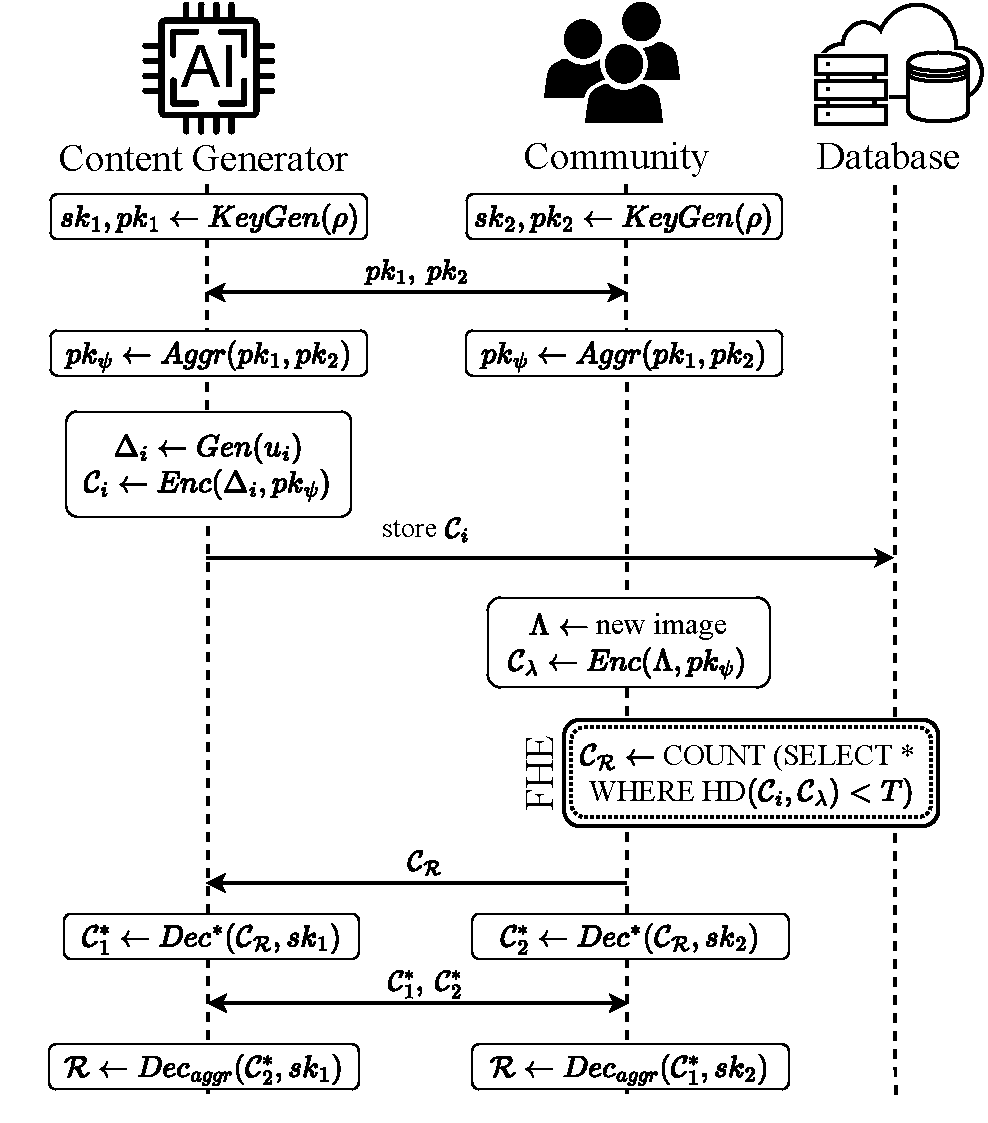
\includegraphics[width=0.9\linewidth,trim={.5cm 0 0 0},clip]{figures/protocol.pdf}
   \caption{\textbf{Overview of the protocol.} The database is kept private, content generators can write encrypted data to it, and the public can run private queries that return only provenance data.}
   \label{fig:protocol}
   \vspace{-0.5cm}
\end{figure}


% In this section we provide a general overview of the proposed architecture. The solution illustrates how a Multi-Party Fully Homomorphic Encryption~(MP-FHE) scheme can be integrated into the Proteus protocol to ensure preserving privacy.

\vspace{-0.5cm}
\paragraph{\textbf{Protocol Details}}
Figure~\ref{fig:protocol} illustrates a scenario involving two parties~(for simplicity) executing a secure protocol: one as the content creator~(the owner of generative model) and the other as a regulator or trusted entity~(a community representative). Each party possesses their own set of private and public keys. The protocol operates in the following four phases:
\begin{compactitem}[-]
    \item \textbf{Setup Phase:} Parties exchange shares of their public keys to create an aggregated $m\mbox{-of-}n$ MPC public key. The shared key is used universally to encrypt pHash values. Note that all parties generating and signing data are incentivized to contribute up to $(n - m)$ live servers to the protocol, so that they can help ensure that they do not decrypt values in the database. More servers means they could affect liveness, and less servers means they have less control over decryption. 
    
    \item \textbf{Encryption Phase:} pHash value of each image is encrypted using the aggregated public key~($P_{shared}$) and stored in database. Original image is then destroyed in a verifiable manner.
    To enhance the accuracy of future claims of copyright violations, parties may decide to also store MPC-encrypted version of each image for a ceremony-based opening under specific conditions, like when pHash matches show very low hamming distance. 
    
    \item \textbf{Evaluation Phase:} When a new image is submitted for evaluation, the pHash value of the image is encrypted using the same shared key~($P_{shared}$) and undergoes a fully homomorphic computation of the Hamming distance across the database. The result is an encrypted output indicating the number of pHash values with close Hamming distances.
    The executed FHE function is merely an example and may vary depending on the specific scenario, database size, or the quality of the pHash values. 
    
    \item \textbf{Decryption Phase:} To decrypt evaluation results, both parties exchange decryption shares in an MPC process. The final value reveals whether the image has any overlaps in the database~(non-zero result) or not~(zero result).
\end{compactitem}

\noindent We implemented our proof-of-concept (PoC) for the proposed system using the \emph{Phantom-Zone} MP-FHE library\footnote{\url{https://github.com/gausslabs/phantom-zone}} in FHEW and link to a comparable implementation of dot product in BFV in Lattigo\footnote{\url{https://eprint.iacr.org/2024/1774.pdf}}. 

\vspace{-0.5cm}\paragraph{\textbf{Method Complexity.}}
The employed MP-FHE scheme supports Boolean operations on encrypted data. For simplicity, we assume each bit of the pHash values is encrypted individually\footnote{In practice, multiple bits are compressed into a single ciphertext to reduce communication and computation complexity}. Thus, for pHash values of length $l$, we have $l$ ciphertexts. \red{However, these ciphertexts are further compressed into a single ciphertext to minimize computational complexity, requiring only a few kilobytes of storage.} Our MP-FHE setup includes a parallel XOR array of length $l$ and a bit-counter of size $l$, which outputs the count of $1$s in an encrypted value. A comparator of size $\log l$ then compares this count with an encrypted threshold value, $Enc(\tau)$, and outputs an encrypted bit: it is $0$ if the Hamming distance exceeds the threshold, indicating a difference above this limit. This comparison process is repeated in parallel for every encrypted value in the registry. Finally, an OR tree with $n$ leaves calculates the OR value of all comparisons, where $n$ is the number of registry entries.
% Assuming $c$ as a constant, the overall complexity for querying one encrypted pHash against the encrypted database is: \textbf{Hamming Distance:} $O(c)$, \textbf{Comparator:} $O(\log l)$, and \textbf{OR tree:} $O(\log n)$, with the OR tree being the dominant factor, making the overall complexity equal to $O(\log n)$.

% \red{We note that as we demonstrate in Section~\ref{sec:benchmarking}, the overall computational cost of }

















One of the key security guarantees of the protocol is that the queries do not leak any information about the dataset, beyond confirming whether the pHash of the query image shares significant similarities with any value in the dataset. To achieve this, we define a set of valid queries that are allowed, with the database managed in an MPC manner.







% There are growing concerns about AI companies and user privacy due to certain prohibited AI practices that pose serious risks to individuals' rights. Due to the General Data Protection Regulation~(GDPR), companies like OpenAI encounter significant challenges when it comes to saving and reusing user data. For example, OpenAI's Advanced Voice mode is unavailable in the EU because the voice data is eligible for zero retention~\cite{OpenAIPolicies}. Thus it is important to design a system for attesting the generated data by AI to preserve copy-right related concerns and both preserve the content owners privacy.
% In this section we provide a general overview of the proposed architecture. The solution illustrates how a Multi-Party Fully Homomorphic Encryption~(MP-FHE) scheme can be integrated into the Proteus protocol to ensure preserving privacy.

% Figure~\ref{fig:protocol} illustrates a scenario involving two parties~(for simplicity) executing a secure protocol: one as the content creator~(e.g., OpenAI) and the other as a regulator or trusted entity~(e.g., a DAO). Each party possesses its own private and public keys, and the protocol operates in four phases:
% \begin{itemize}
%     \item \textbf{Setup Phase:} The parties exchange shares of their public keys to create an aggregated 2-of-2 MPC public key. This shared key is used universally to encrypt images pHash values.
%     \item \textbf{Encryption Phase:} The pHash value of each image is encrypted using the shared public key~($P_{shared}$) and stored in a database. The original image is then destroyed in a verifiable manner??.
%     To enhance the accuracy of claims, the protocol can also store an MPC-encrypted version of the entire original image for ceremony-based opening under specific conditions, such as when pHash matches show high overlaps. 
%     \item \textbf{Evaluation Phase:} When a new image is submitted for evaluation, the pHash value of the image is encrypted using the same shared key~($P_{shared}$) and undergoes a fully homomorphic computation of the Hamming distance across the database. The result is an encrypted output indicating the number of pHash values with close Hamming distances.
%     The executed FHE function is merely an example and may vary depending on the specific scenario, database size, or the quality of the pHash values??. 
%     \item \textbf{Decryption Phase:} To decrypt the evaluation result, both parties exchange their decryption shares in an MPC process. The final value reveals whether the image has any overlaps with the database~(non-zero result) or not~(zero result).
% \end{itemize}


\subsection{Detector for Unknown Images}

\noindent\textbf{Architecture} Open Clip~\cite{ilharco_openclip_2021} has trained various contrastive image-language models with better zero-shot performance on ImageNet \cite{imagenet} than OpenAI's open-sourced version. So, we choose four image encoders for our experiments: SigLIP \cite{zhai2023sigmoid} models with SoViT-400M \cite{alabdulmohsin2024getting} backbone with an input resolution of 224 and 384 and CLIP models with ViT-H \cite{dosovitskiy2020vit} backbone with an input resolution of 224 and 378. We use SVM as our classifier and the second last layer to extract embeddings following \cite{cozzolino2024raising}.

\noindent\textbf{Method} We perform two sets of experiments. 1) We use the better encoders from Open CLIP and train an SVM on the features extracted from their visual encoders. 2) We finetune the entire encoder backbone along with the SVM layer. We follow the technique proposed by \citet{wortsman2022robust} and interpolate between the finetuned and original encoder weights for robustness. We find that the training loss converges significantly within the first two epochs. So, we finetune each model for five epochs and use the validation set to choose the epoch, after which we get the best-performing model. \Cref{tab:training_config} details the number of epochs for which each of the four encoders that were finetuned.

